\chapter{Rysunki}
Wszystkie elementy dokumentu opracowanego w~systemie \LaTeX powinny wyglądać jednolicie. Do wykonywania rysunków korzystamy więc z mechanizmów oferowanych przez dodatkowe pakiety \LaTeX a, nie dołączamy rysunków wykonanych jakościowo różnych, np. wykonanych w~programie Word. Nie używamy rysunkach zapisanych w~plikach bitmapowych, lecz w~plikach wektorowych (\verb+pdf+, ew. \verb+ps+ lub \verb+eps+). Jedynym wyjątkiem są zdjęcia.

\section{Schematy blokowe}
Do opracowania schematów blokowych najlepiej wykorzystać język opisu rysunków \verb+TikZ/PGF+ \cite{litTantau2015}. Przy wykonywaniu prostych rysunków po prostu opisujemy je za pomocą poleceń dodających kolejne elementy, tzn. prostokąty, okręgi, linie. Na przykład, ciąg poleceń:
\begin{lstlisting}[style=customlatex,frame=single] 
\begin{figure}[b]
\centering
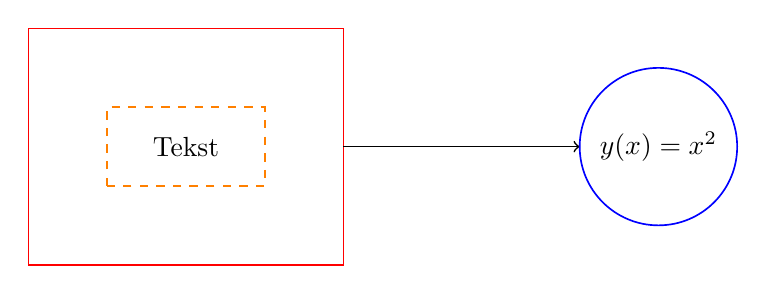
\begin{tikzpicture}
\draw [red, semithick] (0,0) rectangle (4,3);
\draw [orange, semithick,dashed] (1,1) rectangle (3,2);
\draw [->,semithick] (4,1.5) -- (7,1.5);
\draw [blue, semithick] (8,1.5) circle [radius=1];
\node at (2,1.5) {Tekst};
\node at (8,1.5) {$y(x)=x^2$};
\end{tikzpicture}
\end{figure}
\end{lstlisting}
pozwala narysować figury geometryczne przedstawione na rys. \ref{r_tikz_przyklad}. Zwróćmy uwagę, że napis oraz wzór są złożone aktualnie wykorzystywaną czcionką, jej wielkość jest taka sama jak w~całym dokumencie.

\begin{figure}[b]
\centering
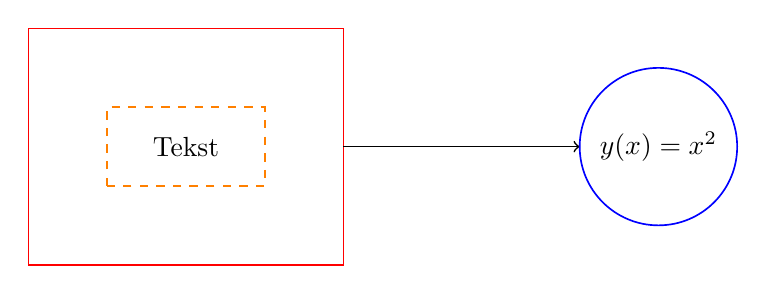
\begin{tikzpicture}
\draw [red, semithick] (0,0) rectangle (4,3);
\draw [orange, semithick,dashed] (1,1) rectangle (3,2);
\draw [->,semithick] (4,1.5) -- (7,1.5);
\draw [blue, semithick] (8,1.5) circle [radius=1];;
\node at (2,1.5) {Tekst};
\node at (8,1.5) {$y(x)=x^2$};
\end{tikzpicture}
%\caption{Przykładowy rysunek wykorzystany w~języku \verb+TikZ/PGF+}
\caption{Tekst Przykładowy rysunek wykorzystany w~języku \texttt{TikZ/PGF}}
\label{r_tikz_przyklad}
\end{figure}

Przy większych rysunkach można wykorzystać programy umożliwiające ich przygotowanie przy wykorzystaniu środowiska graficznego, np. \verb+TikzEdt+ (\url{http://www.tikzedt.org/}), \verb+TpX+ (\url{http://tpx.sourceforge.net/}), \verb+ktikz+ (\url{https://www.linux-apps.com/p/1126914/}), \verb+GraTeX+ (\url{https://sourceforge.net/projects/gratex/}).

Można również wykorzystać starsze, klasyczne pakiety \verb+picture+, \verb+epic+, \verb+eepic+. Również w~tych przypadkach można ,,ręcznie'' opisywać poszczególne elementy graficzne lub skorzystać ze środowiska graficznego, np. \verb+LaTeXPiX+ (\url{http://latexpix.software.informer.com/}), które znacznie przyspiesza pracę. Inne narzędzia, umożliwiające opracowanie rysunków wysokiej jakości, to \verb+METAPOST+ oraz \verb+PSTricks+.

\section{Funkcje statyczne}
Do wykonywania wykresów prezentujących wyniki symulacji i~eksperymentów stosuje się pakiet \verb+PGFPLOTS+ \cite{litFeuersanger2016}. Załóżmy, że w~katalogu \verb+rysunki/dane_stat+ znajduje się plik \verb+dane_fx.txt+ zawierający w~pierwszej kolumnie wartości argumentu $x$, natomiast w~drugiej kolumnie wartości funkcji $f(x)$
\begin{lstlisting}[style=customlatex,frame=single]
  -10.0000 -808.7350
   -9.0000 -696.4791
   -8.0000 -539.7850
   -7.0000 -386.1268
   -6.0000 -291.5881
   -5.0000 -267.6436
   -4.0000 -268.9551
   -3.0000 -233.3995
   -2.0000 -137.5303
   -1.0000  -16.4788
         0   70.0000
    1.0000   94.1212
    2.0000   87.2697
    3.0000  112.8005
    4.0000  209.4449
    5.0000  357.3564
    6.0000  498.0119
    7.0000  589.6732
    8.0000  647.4150
    9.0000  730.9209
   10.0000  891.2650
\end{lstlisting}
oraz podobny plik \verb+dane_gx.txt+, definiujący funkcję $g(x)$. Aby narysować te funkcje stosuje się polecenia:
\begin{lstlisting}[style=customlatex,frame=single]
\begin{figure}[t]
\centering
\begin{tikzpicture}
\begin{axis}[
width=0.5\textwidth,
xmin=-10,xmax=10,ymin=-1000,ymax=1000,
xlabel={$x$},
ylabel={$f(x), \ g(x)$},
xtick={-10,-5,0,5,10},
ytick={-1000,-500,0,500,1000},
legend pos=south east,
y tick label style={/pgf/number format/1000 sep=},
]
\addplot[red,semithick] file {rysunki/dane_stat/dane_fx.txt};
\addplot[blue,semithick,densely dashed]
file {rysunki/dane_stat/dane_gx.txt};
\legend{$f(x)$,$g(x)$}
\end{axis}
\end{tikzpicture}
\caption{Przykładowy rysunek funkcji $f(x)$ i~$g(x)$ wykonany 
w~języku \texttt{PGFPLOTS}}
\label{r_pgfplots_funkcje}
\end{figure}
\end{lstlisting}
Otrzymany rezultat przedstawiono na rys.~\ref{r_pgfplots_funkcje}. Istnieje możliwość ustawienia wielkości czcionek liczb umieszczonych: na osiach (\verb+tick label style+), w~oznaczeniach osi (\verb+label style+), w~legendzie (\verb+legend style+) oraz w~tytule rysunku (\verb+title style+). Przykładowa konfiguracja zmieniająca wielkość czcionek jest następująca:
\begin{lstlisting}[style=customlatex,frame=single]
\pgfplotsset{
tick label style={font=\tiny},
label style={font=\footnotesize},
legend style={font=\footnotesize},
title style={font=\footnotesize}
}
\end{lstlisting}

\begin{figure}[tb]
\centering
\begin{tikzpicture}
\begin{axis}[
width=0.5\textwidth,
xmin=-10,xmax=10,ymin=-1000,ymax=1000,
xlabel={$x$},
ylabel={$f(x), \ g(x)$},
xtick={-10,-5,0,5,10},
ytick={-1000,-500,0,500,1000},
legend pos=south east,
y tick label style={/pgf/number format/1000 sep=},
]
\addplot[red,semithick] file {rysunki/dane_stat/dane_fx.txt};
\addplot[blue,semithick,densely dashed]
file {rysunki/dane_stat/dane_gx.txt};
\legend{$f(x)$,$g(x)$}
\end{axis}
\end{tikzpicture}
\caption{Przykładowy rysunek funkcji $f(x)$ i~$g(x)$ wykonany w~języku \texttt{PGFPLOTS} (rysunek jest kompilowany przy każdym przetworzenia pliku źródłowego}
\label{r_pgfplots_funkcje}
\end{figure}

Opisany sposób implementacji rysunków jest poprawny, ale ma poważną wadę, ponieważ \LaTeX{}   potrzebuje dość dużo czasu na ich przetworzenie. Okazuje się to dużym mankamentem szczególnie wówczas, gdy w~dokumencie znajduje się dużo skomplikowanych rysunków. Skutecznym rozwiązaniem jest przygotowanie rysunków i~zapis ich do plików \verb+pdf+, a~następnie dołączenie ich do głównego dokumentu poleceniem \verb+\includegraphics+. Plik \verb+zapisz_pdf_funkcje.tex+, umożliwiający zapisanie rysunku do pliku \verb+funkcje.pdf+, znajduje się w~katalogu \verb+rysunki/zapisz_pdf+ i~ma następującą postać:
\begin{lstlisting}[style=customlatex,frame=single]
\documentclass[a4paper,11pt]{article}
\usepackage{pgfplots}
\usetikzlibrary{pgfplots.groupplots}
\pgfplotsset{compat=1.11}
\usepgfplotslibrary{external}
\tikzexternalize

\textwidth 160mm \textheight 247mm

\pgfplotsset{width=\figurewidth,compat=1.11}
\pgfplotsset{
tick label style={font=\tiny},
label style={font=\footnotesize},
legend style={font=\footnotesize},
title style={font=\footnotesize}
}

\begin{document}

\tikzsetnextfilename{}

\begin{figure}[tb]
\tikzsetnextfilename{funkcje}
\begin{tikzpicture}
\begin{axis}[
width=0.5\textwidth,
xmin=-10,xmax=10,ymin=-1000,ymax=1000,
xlabel={$x$},
ylabel={$f(x), \ g(x)$},
xtick={-10,-5,0,5,10},
ytick={-1000,-500,0,500,1000},
legend pos=south east,
y tick label style={/pgf/number format/1000 sep=},
]
\addplot[red,semithick] file {../dane_stat/dane_fx.txt};
\addplot[blue,semithick,densely dashed] file {../dane_stat/dane_gx.txt};
\legend{$f(x)$,$g(x)$}
\end{axis}
\end{tikzpicture}
\end{figure}

\end{document}
\end{lstlisting}
Polecenie
\begin{lstlisting}[style=customlatex,frame=single]
pdflatex -shell-escape zapisz_pdf_funkcje.tex
\end{lstlisting}
zapisuje plik \verb+funkcje.pdf+. Umieszczając wiele definicji rysunków w~jednym pliku źródłowym można  generować wiele rysunków w~postaci plików \verb+pdf+. Rysunek dołącza się do dokumentu ciągiem instrukcji:
\begin{lstlisting}[style=customlatex,frame=single]
\begin{figure}[tb]
\centering
\includegraphics[scale=1]{pgfplots_pdf/funkcje}
\caption{Przykładowy rysunek funkcji $f(x)$ i~$g(x)$ wykonany
w~języku \texttt{PGFPLOTS}}
\label{r_pgfplots_funkcje}
\end{figure}
\end{lstlisting}
Otrzymany rezultat przedstawiono na rys.~\ref{r_pgfplots_funkcje_pdf}. Oczywiście, rysunki \ref{r_pgfplots_funkcje} i~\ref{r_pgfplots_funkcje_pdf} są bardzo podobne, jedyną różnicą jest wielkość czcionek.

Nie należy skalować rysunku, gdyż zmieni to wielkość zastosowanej czcionki. Jeżeli zachodzi konieczność zmiany wielkości rysunku, należy zmodyfikować plik źródłowy generujący rysunek.

Jeżeli rysunek jest szerszy niż szerokość strony, należy zastosować otoczenie \verb+sidewaysfigure+ z~pakietu \verb+rotating+, które działa analogicznie jak otoczenie \verb+sidewaystable+.

Przy dużych zbiorach danych \LaTeX{} zgłasza błąd pamięci. Należy wówczas zastosować \hbox{Lua\LaTeX}.

W~bardzo podobny sposób przygotowuje się rysunki trójwymiarowe \cite{litFeuersanger2016}.

\begin{figure}[ptb]
\centering
\includegraphics[scale=1]{rysunki/zapisz_pdf/funkcje}
\caption{Przykładowy rysunek funkcji $f(x)$ i~$g(x)$ wykonany
w~języku \texttt{PGFPLOTS} i~zapisany w~pliku \texttt{funkcje.pdf}}
\label{r_pgfplots_funkcje_pdf}
\end{figure}

\section{Wyniki symulacji i~eksperymentów}
Załóżmy, że w~katalogu \verb+rysunki/symulacje11+ znajduje się plik \verb+yzad.txt+ zawierający w~pierwszej kolumnie pomiary czasu $t$ (w~sekundach), natomiast w~drugiej kolumnie próbki sygnału wartości zadanej $y^{\mathrm{zad}}$. Wykonano symulacje algorytmu regulacji GPC przy pięciu różnych wartościach parametru $\lambda$: $0{,}1$, $0{,}2$, $0{,}5$, $1$ i~$2$. Przebiegi sygnału sterującego $u$ zapisano w~plikach \verb+u_lambda_0_1.txt+, \verb+u_lambda_0_2.txt+, \verb+u_lambda_0_5.txt+, \verb+u_lambda_1.txt+ i~\verb+u_lambda_2.txt+, natomiast przebiegi sygnału wyjściowego procesu $y$ zapisano w~plikach \verb+y_lambda_0_1.txt+, \verb+y_lambda_0_2.txt+, \verb+y_lambda_0_5.txt+, \verb+y_lambda_1.txt+ i~\verb+y_lambda_2.txt+. Przygotowano plik \verb+zapisz_pdf_symulacje11.tex+, umożliwiający zapisanie rysunku do pliku \verb+symulacje11.pdf+. Znajduje się on w~katalogu \verb+rysunki/zapisz_pdf+ i~ma następującą postać:
\begin{lstlisting}[style=customlatex,frame=single]
\documentclass[a4paper,11pt]{article}
\usepackage{pgfplots}
\usetikzlibrary{pgfplots.groupplots}
\pgfplotsset{compat=1.11}
\usepgfplotslibrary{external}
\tikzexternalize

\textwidth 160mm \textheight 247mm

\pgfplotsset{width=\figurewidth,compat=1.11}
\pgfplotsset{
tick label style={font=\tiny},
label style={font=\footnotesize},
legend style={font=\footnotesize},
title style={font=\footnotesize}
}

\newcommand{\szer}{16cm}
\newcommand{\wys}{5.6cm}
\newcommand{\odstepionowy}{1.2cm}

\definecolor{kolor4}{rgb}{0,0,0.1724}
\definecolor{kolor5}{rgb}{1.0000,0.1034,0.7241}
\definecolor{kolor6}{rgb}{1.0000,0.8276,0}

\begin{document}

\tikzsetnextfilename{}

\begin{figure}[tb]
\tikzsetnextfilename{symulacje11}
\begin{tikzpicture}
\begin{groupplot}[group style={group size=1 by 2,vertical sep=\odstepionowy},
width=\szer,height=\wys]
%%1
\nextgroupplot
[xmin=0,xmax=1,ymin=-4.5,ymax=8.5,
xtick={0,0.2,0.4,0.6,0.8,1},ytick={-4,-2,0,2,4,6,8},
xlabel=$t \ (\mathrm{s})$,ylabel=$u$,legend cell align=left,
legend pos=north east]
\addplot[const plot,color=blue,semithick]
file {../symulacje11/u_lambda_0_1.txt};
\addplot[const plot,color=red,semithick,densely dashed]
file {../symulacje11/u_lambda_0_2.txt};
\addplot[const plot,color=green,semithick,densely dashdotted]
file {../symulacje11/u_lambda_0_5.txt};
\addplot[const plot,color=kolor4,semithick,densely dashdotdotted]
file {../symulacje11/u_lambda_1.txt};
\addplot[const plot,color=kolor5,semithick,densely dotted]
file {../symulacje11/u_lambda_2.txt};
\legend{$\lambda=0.1$,$\lambda=0.2$,$\lambda=0.5$,$\lambda=1$,$\lambda=2$}
%%2
\nextgroupplot
[xmin=0,xmax=1,ymin=-1.25,ymax=2.25,
xtick={0,0.2,0.4,0.6,0.8,1},ytick={-1,-0.5,0,0.5,1,1.5,2},
xlabel=$t \ (\mathrm{s})$,ylabel={$y^{\mathrm{zad}}, \ y$},
legend cell align=left,legend style={at={(axis cs:0.6,-0.3)},anchor=south west}]
\addplot[const plot,color=gray,thick]
file {../symulacje11/yzad.txt};
\addplot[color=blue,semithick]
file {../symulacje11/y_lambda_0_1.txt};
\addplot[const plot,color=red,semithick,densely dashed]
file {../symulacje11/y_lambda_0_2.txt};
\addplot[const plot,color=green,semithick,densely dashdotted]
file {../symulacje11/y_lambda_0_5.txt};
\addplot[const plot,color=kolor4,semithick,densely dashdotdotted]
file {../symulacje11/y_lambda_1.txt};
\addplot[const plot,color=kolor5,semithick,densely dotted]
file {../symulacje11/y_lambda_2.txt};
\legend{$y^{\mathrm{zad}}$,$\lambda=0.1$,$\lambda=0.2$,
$\lambda=0.5$,$\lambda=1$,$\lambda=2$}
\end{groupplot}
\end{tikzpicture}
\end{figure}

\end{document}
\end{lstlisting}
Polecenie
\begin{lstlisting}[style=customlatex,frame=single]
pdflatex -shell-escape zapisz_pdf_symulacje11.tex
\end{lstlisting}
zapisuje plik \verb+symulacje11.pdf+. Rysunek dołącza się do dokumentu instrukcją \verb+\includegraphics+. Efekt przedstawiono na rys.~\ref{r_pgfplots_symulacje11_pdf}. Zwróćmy uwagę, że do narysowania wyników symulacji dla kolejnych wartości parametru $\lambda$ zastosowano różne kolory oraz różne style linii (linia ciągła, linia przerywana, itd.). Umożliwia to łatwe rozróżnienie dokumentów na czarno-białym wydruku. Przy wydruku kolorowym oraz dokumentach elektronicznych można zrezygnować ze stosowania różnych stylów linii, do ich rozróżnienia wystarczające są kolory, pod warunkiem jednak, że kolejne krzywe nie są położone bardzo blisko siebie.

Pakiet \verb+PGFPLOTS+ można skonfigurować w~taki sposób, aby na osiach stosowane były liczby z~przecinkiem dziesiętnym w~miejsce kropki dziesiętnej \cite{litFeuersanger2016}.

Czasami ze względu na ograniczoną objętość dokumentu należy zmniejszyć rysunki. Aby zmniejszyć objętość można zastosować ułożenie poziome dwóch rysunków, prezentujących wyniki symulacji procesu. Przygotowano plik \verb+zapisz_pdf_symulacje11_wersja2.tex+, umożliwiający zapisanie rysunku do pliku \verb+symulacje11_wersja2.pdf+. Znajduje się on w~katalogu \verb+rysunki/zapisz_pdf+ i~ma następującą postać:
\begin{lstlisting}[style=customlatex,frame=single]
\documentclass[a4paper,11pt]{article}
\usepackage{pgfplots}
\usetikzlibrary{pgfplots.groupplots}
\pgfplotsset{compat=1.11}
\usepgfplotslibrary{external}
\tikzexternalize

\textwidth 160mm \textheight 247mm

\pgfplotsset{width=\figurewidth,compat=1.11}
\pgfplotsset{
tick label style={font=\tiny},
label style={font=\footnotesize},
legend style={font=\footnotesize},
title style={font=\footnotesize}
}

\newcommand{\szer}{8cm}
\newcommand{\wys}{5.6cm}
\newcommand{\odstepoziomy}{1.9cm}

\definecolor{kolor4}{rgb}{0,0,0.1724}
\definecolor{kolor5}{rgb}{1.0000,0.1034,0.7241}
\definecolor{kolor6}{rgb}{1.0000,0.8276,0}

\begin{document}

\tikzsetnextfilename{}

\begin{figure}[tb]
\tikzsetnextfilename{symulacje11_wersja2}
\begin{tikzpicture}
\begin{groupplot}[group style={group size=2 by 1,horizontal sep=\odstepoziomy},
width=\szer,height=\wys]
%%1
\nextgroupplot
[xmin=0,xmax=1,ymin=-4.5,ymax=8.5,
xtick={0,0.2,0.4,0.6,0.8,1},ytick={-4,-2,0,2,4,6,8},
xlabel=$t \ (\mathrm{s})$,ylabel=$u$,,legend style={at={(0,1.15)},anchor=west},
legend columns=6,legend style={/tikz/every even column/.append style=
{column sep=1.4cm}}]
\addplot[const plot,color=blue,semithick]
file {../symulacje11/u_lambda_0_1.txt};
\addplot[const plot,color=red,semithick,densely dashed]
file {../symulacje11/u_lambda_0_2.txt};
\addplot[const plot,color=green,semithick,densely dashdotted]
file {../symulacje11/u_lambda_0_5.txt};
\addplot[const plot,color=kolor4,semithick,densely dashdotdotted]
file {../symulacje11/u_lambda_1.txt};
\addplot[const plot,color=kolor5,semithick,densely dotted]
file {../symulacje11/u_lambda_2.txt};
\legend{$\lambda=0.1$,$\lambda=0.2$,$\lambda=0.5$,$\lambda=1$,$\lambda=2$}
%%2
\nextgroupplot
[xmin=0,xmax=1,ymin=-1.25,ymax=2.25,
xtick={0,0.2,0.4,0.6,0.8,1},ytick={-1,-0.5,0,0.5,1,1.5,2},
xlabel=$t \ (\mathrm{s})$,ylabel={$y^{\mathrm{zad}}, \ y$},
legend cell align=left]
\addplot[const plot,color=gray,thick] file {../symulacje11/yzad.txt};
\addplot[color=blue,semithick] file {../symulacje11/y_lambda_0_1.txt};
\addplot[const plot,color=red,semithick,densely dashed]
file {../symulacje11/y_lambda_0_2.txt};
\addplot[const plot,color=green,semithick,densely dashdotted]
file {../symulacje11/y_lambda_0_5.txt};
\addplot[const plot,color=kolor4,semithick,densely dashdotdotted]
file {../symulacje11/y_lambda_1.txt};
\addplot[const plot,color=kolor5,semithick,densely dotted]
file {../symulacje11/y_lambda_2.txt};
\legend{$y^{\mathrm{zad}}$}
\end{groupplot}
\end{tikzpicture}
\end{figure}

\end{document}

\end{lstlisting}
Rysunek dołącza się do dokumentu instrukcją \verb+\includegraphics+. Efekt przedstawiono na rys.~\ref{r_pgfplots_symulacje11_wersja2_pdf}.

\begin{figure}[tb]
\centering
\includegraphics[scale=1]{rysunki/zapisz_pdf/symulacje11}
%\includegraphics[scale=1]{rysunki/zapisz_pdf/symulacje11}
\caption{Przykładowy rysunek wyników symulacji procesu jednowymiarowego wykonany
w~języku \texttt{PGFPLOTS} i~zapisany w~pliku \texttt{symulacje11.pdf}}
\label{r_pgfplots_symulacje11_pdf}
\end{figure}

\begin{figure}[tb]
\centering
\includegraphics[scale=1]{rysunki/zapisz_pdf/symulacje11_wersja2}
\caption{Przykładowy rysunek wyników symulacji procesu jednowymiarowego wykonany
w~języku \texttt{PGFPLOTS} i~zapisany w~pliku \texttt{symulacje11\_wersja2.pdf}}
\label{r_pgfplots_symulacje11_wersja2_pdf}
\end{figure}

Załóżmy, że w~katalogu \verb+rysunki/symulacje22+ znajdują się wyniki symulacji procesu o~dwóch wejściach i~dwóch wyjściach zapisane w~plikach: \verb+u1.txt+, \verb+u2.txt+, \verb+y1.txt+, \verb+y2.txt+, \verb+yzad1.txt+, \verb+yzad2.txt+. W~pierwszej kolumnie tych plików podano czas $t$ (w~sekundach), natomiast w~drugiej kolumnie wartość odpowiedniej zmiennej. Plik \verb+zapisz_pdf_symulacje22.tex+, umożliwiający zapisanie rysunku do pliku \verb+symulacje22.pdf+ znajduje się w~katalogu \verb+rysunki/zapisz_pdf+ i~ma następującą postać:
\begin{lstlisting}[style=customlatex,frame=single]
\documentclass[a4paper,11pt]{article}
\usepackage{pgfplots}
\usetikzlibrary{pgfplots.groupplots}
\pgfplotsset{compat=1.11}
\usepgfplotslibrary{external}
\tikzexternalize

\textwidth 160mm \textheight 247mm

\pgfplotsset{width=\figurewidth,compat=1.11}
\pgfplotsset{
tick label style={font=\tiny},
label style={font=\footnotesize},
legend style={font=\footnotesize},
title style={font=\footnotesize}
}

\newcommand{\szer}{16cm}
\newcommand{\wys}{6cm}
\newcommand{\odstepionowy}{1.2cm}

\begin{document}

\tikzsetnextfilename{}

\begin{figure}[tb]
\tikzsetnextfilename{symulacje22}
\begin{tikzpicture}
\begin{groupplot}[group style={group size=1 by 4,vertical sep=\odstepionowy},
width=\szer,height=\wys]
%%1
\nextgroupplot
[xmin=0,xmax=1,ymin=-0.1,ymax=3,
xtick={0,0.2,0.4,0.6,0.8,1},ytick={0,1,2,3},
xlabel=$t \ (\mathrm{s})$,ylabel=$u_1$,legend cell align=left,
legend pos=north east]
\addplot[const plot,color=blue,semithick] file {../symulacje22/u1.txt};
%%2
\nextgroupplot
[xmin=0,xmax=1,ymin=-0.5,ymax=1.5,
xtick={0,0.2,0.4,0.6,0.8,1},ytick={-0.5,0,0.5,1,1.5},
xlabel=$t \ (\mathrm{s})$,ylabel=$u_2$,legend cell align=left,
legend pos=north east]
\addplot[const plot,color=blue,semithick] file {../symulacje22/u2.txt};
%%3
\nextgroupplot
[xmin=0,xmax=1,ymin=-0.25,ymax=1.5,
xtick={0,0.2,0.4,0.6,0.8,1},ytick={0,0.5,1,1.5},
xlabel=$t \ (\mathrm{s})$,ylabel={$y_1^{\mathrm{zad}}, \ y_1$},
legend cell align=left,legend pos=north east]
\addplot[const plot,color=gray,thick] file {../symulacje22/yzad1.txt};
\addplot[color=blue,semithick] file {../symulacje22/y1.txt};
\legend{$y_1^{\mathrm{zad}}$,$y_1$}
%%4
\nextgroupplot
[xmin=0,xmax=1,ymin=-0.25,ymax=1.5,
xtick={0,0.2,0.4,0.6,0.8,1},ytick={0,0.5,1,1.5},
xlabel=$t \ (\mathrm{s})$,ylabel={$y_2^{\mathrm{zad}}, \ y_2$},
legend cell align=left,legend pos=north east]
\addplot[const plot,color=gray,thick] file {../symulacje22/yzad2.txt};
\addplot[color=blue,semithick] file {../symulacje22/y2.txt};
\legend{$y_2^{\mathrm{zad}}$,$y_2$}
\end{groupplot}
\end{tikzpicture}
\end{figure}

\end{document}
\end{lstlisting}
Rysunek dołącza się do dokumentu instrukcją \verb+\includegraphics+. Efekt przedstawiono na rys.~\ref{r_pgfplots_symulacje22_pdf}.

Aby zmniejszyć objętość można nieco inaczej ułożyć 4 rysunki, prezentujące wyniki symulacji procesu dwuwymiarowego. Przygotowano plik \verb+zapisz_pdf_symulacje2_wersja2.tex+, umożliwiający zapisanie rysunku do pliku \verb+symulacje22_wersja2.pdf+. Znajduje się on w~katalogu \verb+rysunki/zapisz_pdf+ i~ma następującą postać:
\begin{lstlisting}[style=customlatex,frame=single]
\documentclass[a4paper,11pt]{article}
\usepackage{pgfplots}
\usetikzlibrary{pgfplots.groupplots}
\pgfplotsset{compat=1.11}
\usepgfplotslibrary{external}
\tikzexternalize

\textwidth 160mm \textheight 247mm

\pgfplotsset{width=\figurewidth,compat=1.11}
\pgfplotsset{
tick label style={font=\tiny},
label style={font=\footnotesize},
legend style={font=\footnotesize},
title style={font=\footnotesize}
}

\newcommand{\szer}{8cm}
\newcommand{\wys}{5.6cm}
\newcommand{\odstepionowy}{1.2cm}
\newcommand{\odstepoziomy}{1.9cm}

\begin{document}

\tikzsetnextfilename{}

\begin{figure}[tb]
\tikzsetnextfilename{symulacje22_wersja2}
\begin{tikzpicture}
\begin{groupplot}[group style={group size=2 by 2,horizontal sep=\odstepoziomy,
vertical sep=\odstepionowy},width=\szer,height=\wys]
%%1
\nextgroupplot
[xmin=0,xmax=1,ymin=-0.1,ymax=3,
xtick={0,0.2,0.4,0.6,0.8,1},ytick={0,1,2,3},
xlabel=$t \ (\mathrm{s})$,ylabel=$u_1$,legend cell align=left,
legend pos=north east]
\addplot[const plot,color=blue,semithick] file {../symulacje22/u1.txt};
%%2
\nextgroupplot
[xmin=0,xmax=1,ymin=-0.25,ymax=1.5,
xtick={0,0.2,0.4,0.6,0.8,1},ytick={0,0.5,1,1.5},
xlabel=$t \ (\mathrm{s})$,ylabel={$y_1^{\mathrm{zad}}, \ y_1$},
legend cell align=left,legend pos=south east]
\addplot[const plot,color=gray,thick] file {../symulacje22/yzad1.txt};
\addplot[color=blue,semithick] file {../symulacje22/y1.txt};
\legend{$y_1^{\mathrm{zad}}$,$y_1$}
%%3
\nextgroupplot
[xmin=0,xmax=1,ymin=-0.5,ymax=1.5,
xtick={0,0.2,0.4,0.6,0.8,1},ytick={-0.5,0,0.5,1,1.5},
xlabel=$t \ (\mathrm{s})$,ylabel=$u_2$,legend cell align=left,
legend pos=north east]
\addplot[const plot,color=blue,semithick] file {../symulacje22/u2.txt};
%%4
\nextgroupplot
[xmin=0,xmax=1,ymin=-0.25,ymax=1.5,
xtick={0,0.2,0.4,0.6,0.8,1},ytick={0,0.5,1,1.5},
xlabel=$t \ (\mathrm{s})$,ylabel={$y_2^{\mathrm{zad}}, \ y_2$},
legend cell align=left,legend pos=south east]
\addplot[const plot,color=gray,thick] file {../symulacje22/yzad2.txt};
\addplot[color=blue,semithick] file {../symulacje22/y2.txt};
\legend{$y_2^{\mathrm{zad}}$,$y_2$}
\end{groupplot}
\end{tikzpicture}
\end{figure}

\end{document}

\end{lstlisting}
Rysunek dołącza się do dokumentu instrukcją \verb+\includegraphics+. Efekt przedstawiono na rys.~\ref{r_pgfplots_symulacje22_wersja2_pdf}.

\begin{figure}[p]
\centering
\includegraphics[scale=1]{rysunki/zapisz_pdf/symulacje22}
\caption{Przykładowy rysunek wyników symulacji procesu dwuwymiarowego wykonany
w~języku \texttt{PGFPLOTS} i~zapisany w~pliku \texttt{symulacje22.pdf}}
\label{r_pgfplots_symulacje22_pdf}
\end{figure}

\begin{figure}[b]
\centering
\includegraphics[scale=1]{rysunki/zapisz_pdf/symulacje22_wersja2}
\caption{Przykładowy rysunek wyników symulacji procesu dwuwymiarowego wykonany
w~języku \texttt{PGFPLOTS} i~zapisany w~pliku \texttt{symulacje22\_wersja2.pdf}}
\label{r_pgfplots_symulacje22_wersja2_pdf}
\end{figure}

W~katalogu \verb+rysunki/symulacje43+ znajdują się wyniki symulacji procesu o~czterech wejściach i~trzech wyjściach zapisane w~plikach: \verb+u1.txt+, \verb+u2.txt+, \verb+u3.txt+, \verb+u4.txt+, \verb+y1.txt+, \verb+y2.txt+, \verb+y3.txt+, \verb+y1zad.txt+, \verb+y2zad.txt+, \verb+y3zad.txt+. W~pierwszej kolumnie tych plików podano czas $t$ (w~sekundach), natomiast w~drugiej kolumnie wartość odpowiedniej zmiennej. W~katalogu \verb+rysunki/zapisz_pdf+ znajduje się plik \verb+zapisz_pdf_symulacje43.tex+, który zapisuje dwa pliki zawierające wyniki symulacji: \verb+symulacje43u.pdf+ (sygnały sterujące) oraz \verb+symulacje43y.pdf+ (sygnały wartości zadanych oraz sygnały wyjść procesu). Oba rysunki dołącza się do dokumentu dwoma instrukcjami \verb+\includegraphics+, między rysunkami wstawiono niewielki odstęp. Efekt przedstawiono na rys.~\ref{r_pgfplots_symulacje43_pdf}.

\begin{figure}[b]
\centering
\includegraphics[scale=1]{rysunki/zapisz_pdf/symulacje43u}\hspace{3mm}\includegraphics[scale=1]{rysunki/zapisz_pdf/symulacje43y}
\caption{Przykładowy rysunek wyników symulacji procesu o~czterech wejściach i~trzech wyjściach wykonany
w~języku \texttt{PGFPLOTS} i~zapisany w~plikach \texttt{symulacje43u.pdf} oraz \texttt{symulacje43y.pdf}}
\label{r_pgfplots_symulacje43_pdf}
\end{figure}

\section{Kolory}
Przy umieszczaniu kilku wykresów na tym samym rysunku należy zastosować kolory różniące się od siebie w~znacznym stopniu, nie można stosować kolorów podobnych, np. kilku odcieni tego samego koloru. Do generacji palety kolorów spełniającej takie wymagania można użyć funkcji \verb+distinguishable_colors.m+, udostępnionej na stronie \url{https://www.mathworks.com/matlabcentral/}. Zestaw dwudziestu kolorów został przedstawiony na rys.~\ref{r_zestaw_kolorow}. Ich definicja w~palecie RGB jest następująca:
\begin{lstlisting}[style=customlatex,frame=single]
         0         0    1.0000
    1.0000         0         0
         0    1.0000         0
         0         0    0.1724
    1.0000    0.1034    0.7241
    1.0000    0.8276         0
         0    0.3448         0
    0.5172    0.5172    1.0000
    0.6207    0.3103    0.2759
         0    1.0000    0.7586
         0    0.5172    0.5862
         0         0    0.4828
    0.5862    0.8276    0.3103
    0.9655    0.6207    0.8621
    0.8276    0.0690    1.0000
    0.4828    0.1034    0.4138
    0.9655    0.0690    0.3793
    1.0000    0.7586    0.5172
    0.1379    0.1379    0.0345
    0.5517    0.6552    0.4828
\end{lstlisting}
\definecolor{kolor5}{rgb}{1.0000,0.1034,0.7241}
Oprócz kolorów standardowych oraz dodatkowych, które są zdefiniowane w~pakiecie \verb+xcolor+, własne kolory definiujemy poleceniem \verb+\definecolor+. Na przykład, piąty kolor z~zestawu definiujemy poleceniem \verb+\definecolor{kolor5}{rgb}{1.0000,0.1034,0.7241}+, {\color{kolor5}co umożliwia osiągnięcie następującego efektu}.

\begin{figure}[b]
\centering
\includegraphics[width=0.75\textwidth,height=0.1\textheight]{rysunki/kolory}
\caption{Paleta 20 kolorów}
\label{r_zestaw_kolorow}
\end{figure}

\section{Lokalizacja rysunków (i~tabel)}
Wszystkie rysunki i~tabele umieszczamy jako ,,pływające", a~więc w otoczeniu \verb+figure+ oraz \verb+table+ nie stosujemy opcji \verb+[h]+ i~\verb+[H]+. Aby uniknąć umieszczenia rysunków w~tekście kolejnego rozdziału należy zastosować polecenie \verb+\FloatBarrier+ z~pakietu \verb+placeins+.


